% !Mode:: "TeX:UTF-8"
\chapter{硬件框架的设计与搭建}

本章详细描述了本课题硬件框架的设计与搭建,本模块是系统实际落地的硬件基础。本模块的主要工作包括电路设计,模型设计与搭建,轴间对齐,布线优化等。

\section{硬件设备介绍}

\subsection{Arduino Nano开发板}

本魔方复原系统使用Arduino Nano开发板作为下位机。Arduino Nano 是一款基于 ATmega328P的开发板,与Arduino Uno十分类似。它与Uno的区别是Nano没有直流电压供电接口同时Nano通过Mini-B USB 接口与电脑连接,并且Nano的尺寸更加小巧。表~\ref{tab:2-1}、图~\ref{fig:2-1}~与图~\ref{fig:2-2}~分别是Arduino Nano开发板的参数表、实物图和引脚说明图。

\begin{table}[H]
	\caption{主要技术参数}\label{tab:2-1}
	\vspace{0.5em}
	\begin{center}
		{\wuhao
			\begin{tabular}{ccccc}
				\toprule
				属性 & 属性值	\\
				\midrule
				工作电压 & 5伏特 \\
				Flash Memory(闪存) & 32 KB (ATmega328P)\\
				SRAM(静态存储器) & 2 KB (ATmega328P)\\
				EEPROM & 1 KB (ATmega328P)\\
				模拟输入引脚	& 8个\\
				输入/输出引脚直流电流	& 40 毫安\\
				输入电压 & 7-12伏特\\
				数字输入输出引脚 & 22个\\
				PWM引脚 & 6个\\
				3.3V引脚电流 & 50 毫安\\
				长 & 45 mm\\
				宽 & 18 mm\\
				重 & 7克\\
				时钟频率 & 16 MHz\\
				\bottomrule
		\end{tabular}}
	\end{center}
	\vspace{-1.5em}
\end{table}

\begin{figure}[H]
	\centering
	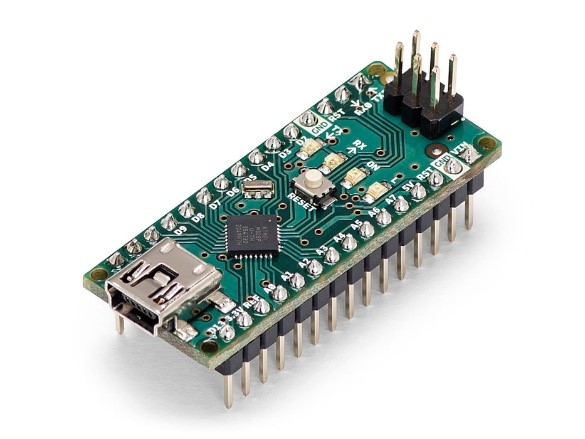
\includegraphics[width=0.8\textwidth]{2-1}
	\caption{Arduino Nano实物图}\label{fig:2-1}
\end{figure}

\begin{figure}[H]
	\centering
	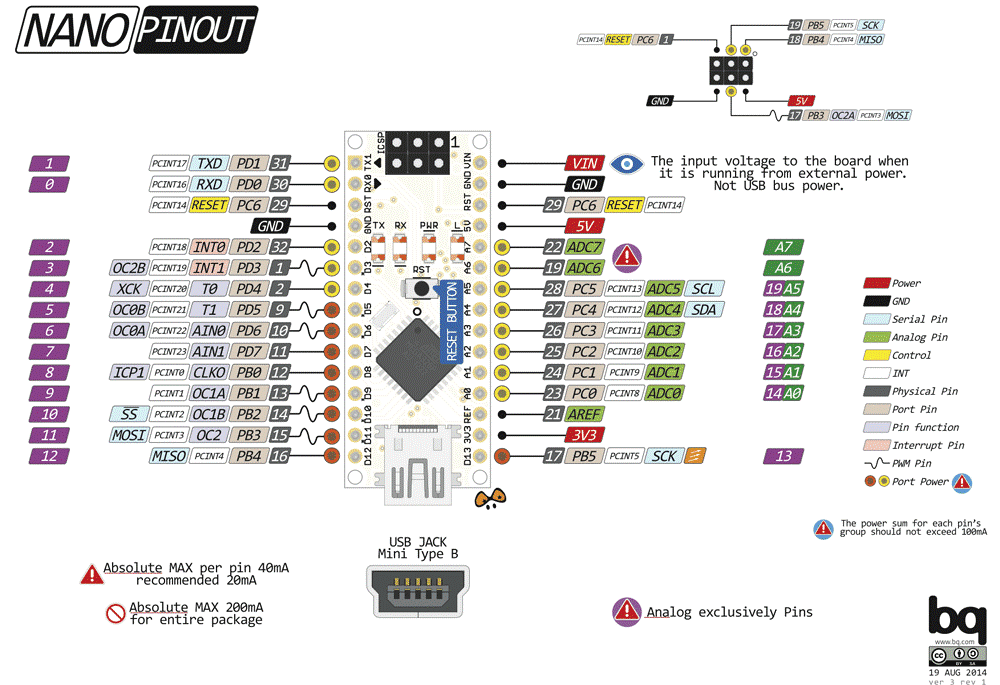
\includegraphics[width=0.9\textwidth]{2-2}
	\caption{引脚说明图}\label{fig:2-2}
\end{figure}

\subsection{SERVO42A闭环步进电机}

步进电机是通过脉冲信号来进行控制,每输入一个脉冲信号,步进电机前进一步。步进电机旋转的步距角,是在电机结构的基础上等比例控制产生的,如果控制电路的细分控制不变,那么步进旋转的步距角在理论上是一个固定的角度。这正好符号了魔方面旋转需要固定角度旋转的特性。


闭环步进电机与普通步进电机的区别在于闭环步进电机的闭环控制采用位置反馈或速度反馈~\cite{26}的方法来确定与转子位置相适应的相位转换~\cite{27},其目的是检测旋转的每一步是否都顺利完成,换言之是为了防止丢步。闭环电机如果出现丢步的情况,自身会通过反馈回电路的信息再补上,原用于生产精度要求比较高的3D打印机,考虑到其精度高,因此将其用于控制魔方面的旋转。

\begin{figure}[H]
	\centering
	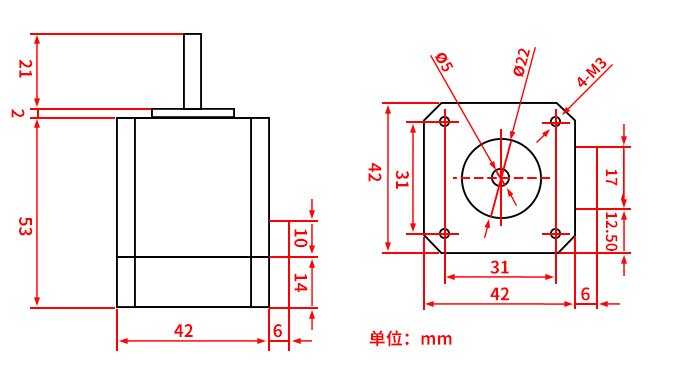
\includegraphics[width=0.5\textwidth]{2-3}
	\caption{SERVO42A电机尺寸图}\label{fig:2-3}
\end{figure}

\begin{figure}[H]
	\centering
	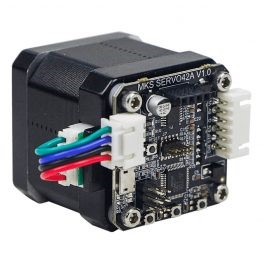
\includegraphics[width=0.5\textwidth]{2-4}
	\caption{SERVO42A电机实物图}\label{fig:2-4}
\end{figure}

闭环控制的步进电机系统或可在具有给定精确度下跟踪和反馈时,扩大工作速度范围,或可在给定速度下提高跟踪和定位精度,或可得到极限速度指标和极限精度指标。步进电机的闭环驱动很有意义,可实现完全无过冲的位置定位,在中低速应用中超越传统电机而取得一定的应用优势,最简单的闭环控制是在常规驱动器外加一个闭环控制器,使磁极磁通与电流的相位关系保持一致,产生能带动负载转矩的电磁转矩,除此之外,更加严格的闭环控制是以控制激磁磁通与电流相位角的方式对步进电机实施矢量控制,称作功率角闭环控制方法。不论哪种闭环控制方法,都可以大幅度提高顺滑性,降低功耗和固有震动。下表~\ref{tab:2-2}~是SERVO42A闭环步进电机的参数表。

\begin{table}[H]
	\caption{电机参数}\label{tab:2-2}
	\vspace{0.5em}
	\begin{center}
		{\wuhao
			\begin{tabular}{ccccc}
				\toprule
				属性 & 属性值	\\
				\midrule
				输入电压 & $12V-24V$\\
				峰值输出电流 & $\pm2A$\\
				闭环反馈频率 & $6kHz$\\
				精度 & $> 0.1125 ^{\circ} $\\
				细分步数 & $16,32,64,128,256$\\
				电机相数 & $2$\\
				保持转矩 & $\ge400mN \cdot m$\\
				转动惯量 & $62.5g \cdot cm^2$\\
				步距角 & $1.8^{\circ} \pm 5\% $ \\
				额定电流 & DC 1.0A/相\\
				\bottomrule
		\end{tabular}}
	\end{center}
	\vspace{-1.5em}
\end{table}

本系统选用闭环步进电机作为魔方一对一旋转的硬件部分,即一台闭环步进电机与一个魔方面相连接,同时,电机实现对魔方面的旋转控制意味着电机的旋转需要精确的位置控制。与开环步进电机相比,闭环步进电机最大的优势在于其高精度性,可稳定地进行旋转操作,具有更高的运行速度,更稳定、更光滑的转速。

\subsection{DS3120伺服电机}
伺服电机是一种传统的电机,在自动控制系统中用作执行元件。该电机可以控制速度,位置精度非常准确,可以将电压信号转化为转矩和转速以驱动控制对象。

伺服电机的转子转速受输入信号控制,并能快速反应,在自动控制系统中,用作执行元件,且具有机电时间常数小、线性度高等特性,可把所收到的电信号转换成电动机轴上的角位移或角速度输出。其主要作用是随着电压的变化控制转速均匀稳定。

伺服电机之所以精度非常准确,是因为靠脉冲来定位,当接受到一个脉冲电流,就会相应的旋转一个脉冲的对应角度,因为伺服电机本身也具有发出脉冲电流的功能,每当旋转一个角度都会发出对应数量的脉冲,和伺服电机接受的脉冲形成了呼应,或者叫闭环,因此能够精确的控制电机的转动,精确的定位可以达到0.001mm。

\begin{figure}[H]
	\centering
	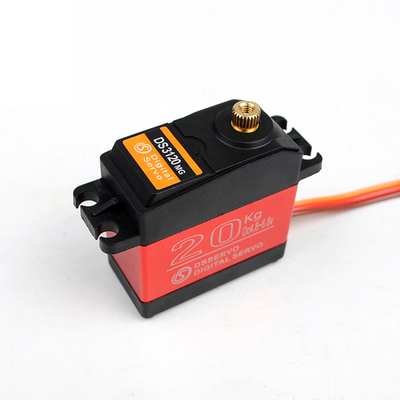
\includegraphics[width=0.4\textwidth]{2-5}
	\caption{伺服电机}\label{fig:2-5}
\end{figure}

与上一部分提到的闭环步进电机相比,伺服电机的精度更高,但是因为考虑到本系统需要同时考虑旋转速度,而伺服电机的旋转速度与闭环步进电机相差较大,因此并不能用于魔方面旋转。在本魔方还原系统中,伺服电机的作用在于将六个步进电机同时向位于中心的魔方移动,稳定魔方的位置,使其紧扣魔方中心块。


\section{六轴架构设计}
现有双臂解魔方机器人系统~\cite{10}~\cite{11}、四臂魔方还原系统~\cite{12}分别采用的是二轴、四轴的方式还原,而非六轴旋转还原的方式存在着单个旋转步骤需要分解为多个电机的旋转操作的缺点。两臂二指魔方机器人如下图~\ref{fig:2-6}~所示。

\begin{figure}[H]
	\centering
	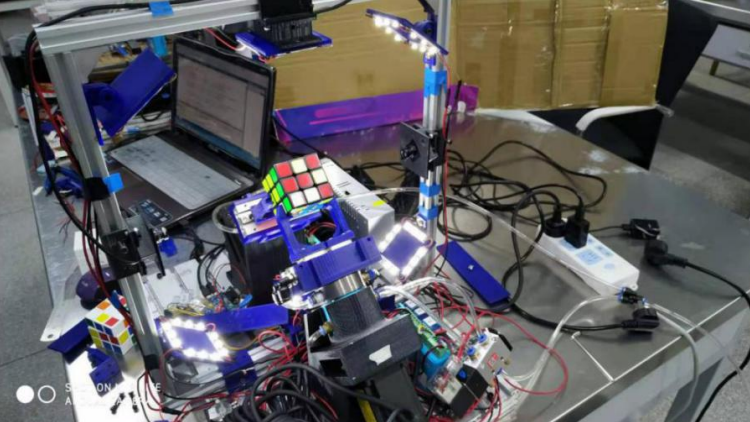
\includegraphics[width=0.8\textwidth]{2-6}
	\caption{两臂二轴魔方机器人}\label{fig:2-6}
\end{figure}

下图~\ref{fig:2-7}~是魔方建立三维坐标系后的示意图。以上述二轴魔方复原系统为例,假设该系统的两个旋转臂分别处于X轴正方向与Y轴正方向。此时若要还原魔方需要对Z轴正方向顺时针旋转 90° 。假设在二轴复原架构下,首先需要将X轴正方向的旋转臂顺时针旋转 90° ,将白色魔方面旋转至Y轴正方向,接着再将顺时针旋转Y轴正方向的旋转臂,两步操作后可复原魔方。但在本论文所设计的六轴复原架构下,只需要将位于Z轴正方向的电机顺时针旋转 90° 一步操作即可完成魔方复原。

也就是说,当需要旋转除与两臂直接接触的魔方面时,都需要进行额外的旋转操作,这将会大大增加魔方复原所消耗的时间,而这些冗余的时间也正是本论文提到的六轴复原架构所能节省的复原时间。

\begin{figure}[H]
	\centering
	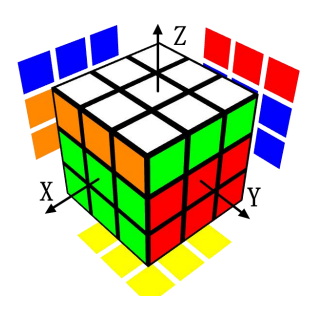
\includegraphics[width=0.55\textwidth]{2-7}
	\caption{带坐标轴的魔方示意图}\label{fig:2-7}
\end{figure}

六轴复原架构的具体实现方法是通过“爪子”将魔方中心块与电机一对一相连接,“爪子”与中心块的凹陷处紧扣后即可通过“爪子”的旋转带动魔方面的旋转。下列左图展示的是魔方中心块示意图,图中中心有四个小凹槽,分别与“爪子”四个凸起部分相匹配,右图是凹槽与“爪子”与红色魔方面相扣时的装配图。

\begin{figure}[H]
	\centering
	\subfigure{
\includegraphics[height=5cm]{2-8}}
%	\hfill
	\subfigure{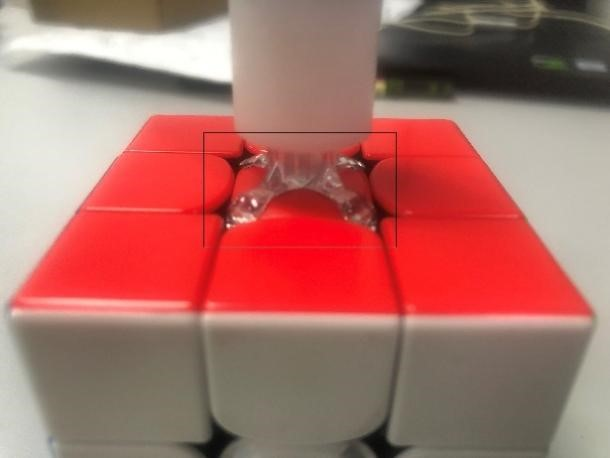
\includegraphics[height=5cm]{2-8.1}}
	\caption{魔方中心块示意图与装配图}\label{fig:2-8}
\end{figure}
本论文提出的六轴复原架构将魔方的六个面均采用上述“爪子”与魔方块一对一紧扣的方式相连接,该架构大大增加了系统的稳定性以及复原速度。

\section{PCB电路板设计}

为了使本魔方复原系统高度集成化,因此自主设计PCB电路板。

PCB电路板是将Arduino Nano下位机与闭环步进电机联结为一体的中间桥梁。该电路板外接12V适配器并搭配降压模块可同时分别向舵机提供5V电压,向步进电机提供12V电压。

此外,通过定义引脚以及电路板连线,将Arduino Nano发送旋转信号的引脚与相应电机的引脚相连接。电路板设计图与实物图如下图~\ref{fig:2-9}~所示,其中实物图左侧的蓝色模块为12V降压模块,可将12V电压降至5V电压,给舵机提供稳定5V电压。

\begin{figure}[H]
	\centering
	\subfigure[电路板设计图]{\label{fig:subfig:2-9}
		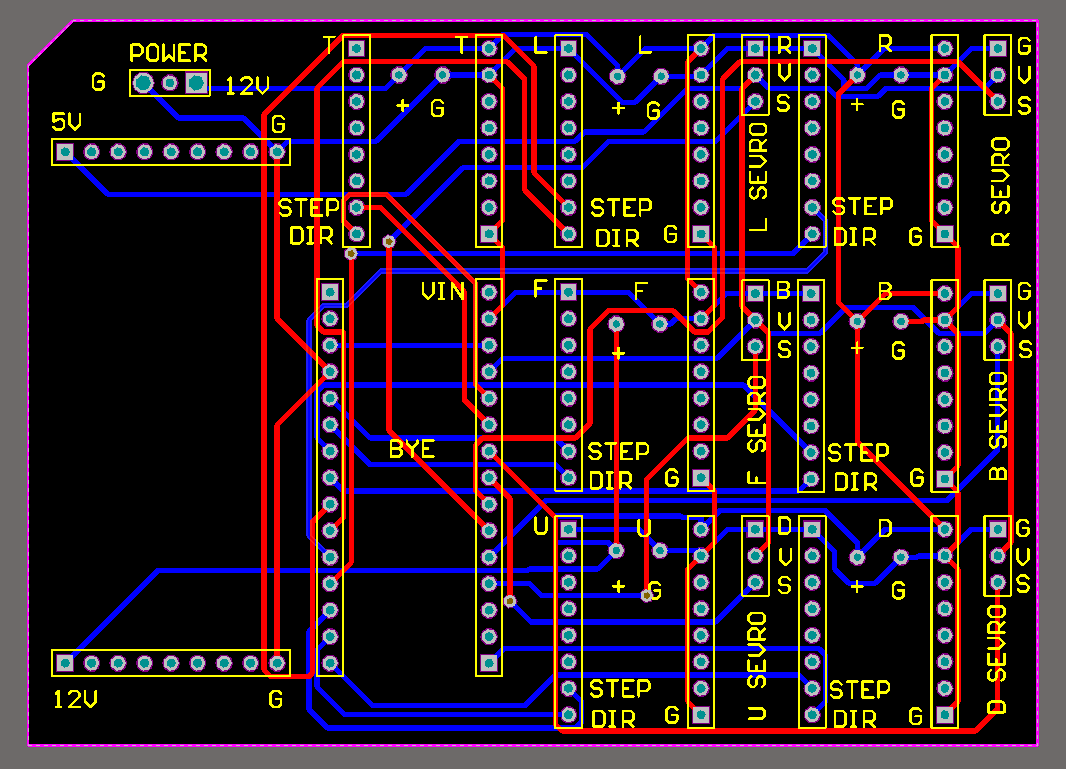
\includegraphics[height=5cm]{2-9}}
	\subfigure[电路板实物图]{\label{fig:subfig:2-9.1}
		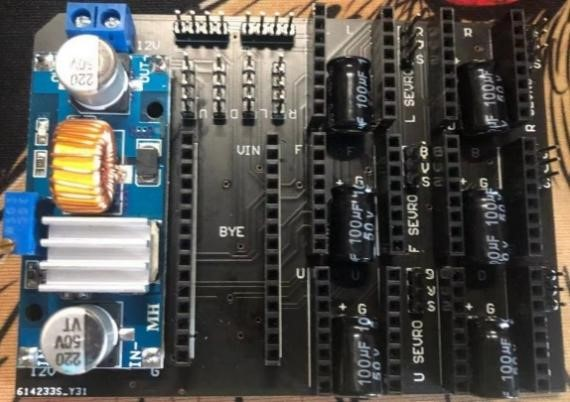
\includegraphics[height=5cm]{2-9.1}}
	\caption{电路板设计图与实物图}\label{fig:2-9}
\end{figure}

\section{三维建模结果图}

\subsection{零件仿真图}

本系统在三维建模阶段所用到的软件为SolidWorks2016,以下图~\ref{fig:2-10}~至图~\ref{fig:2-14}~为三维建模的仿真结果图。每个零件在系统中都有其独一无二、不可取代的作用。其中,图~\ref{fig:2-10}~所示的铝型材作为系统骨架,用于支撑整个系统;图~\ref{fig:2-11}~所示的滑轨用于平行移动步进电机,在伺服电机的驱动下可划动使其夹紧魔方;图~\ref{fig:2-12}~所示的滑块用于承载闭环其上方的步进电机,与图~\ref{fig:2-11}~的滑轨相配合;图~\ref{fig:2-13}~为步进电机与滑块的连接件,用于固定步进电机与滑块;图~\ref{fig:2-14}~为魔方托槽,用于放置本系统未运行状态时的魔方。

\begin{figure}[H]
	\centering
	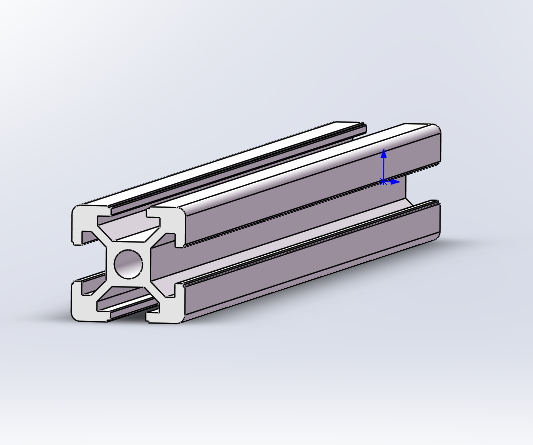
\includegraphics[width=0.6\textwidth]{2-10}
	\caption{铝型材仿真图}\label{fig:2-10}
\end{figure}

\begin{figure}[H]
	\centering
	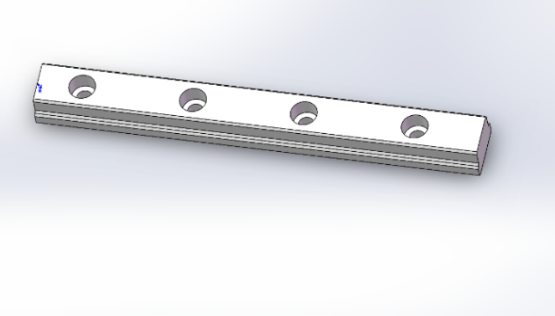
\includegraphics[width=0.6\textwidth]{2-11}
	\caption{滑轨仿真图}\label{fig:2-11}
\end{figure}

\begin{figure}[H]
	\centering
	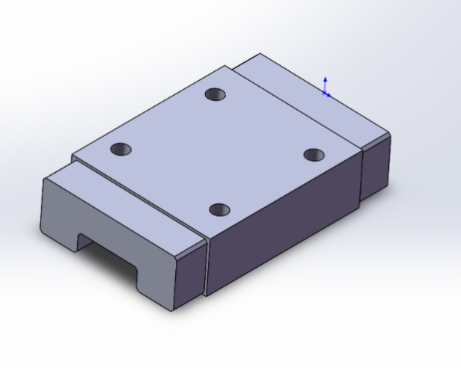
\includegraphics[width=0.6\textwidth]{2-12}
	\caption{滑块仿真图}\label{fig:2-12}
\end{figure}


\begin{figure}[H]
	\centering
	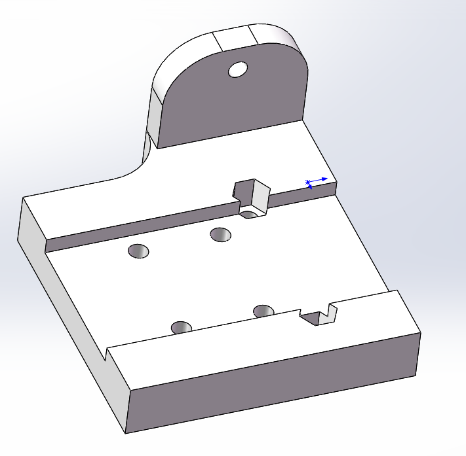
\includegraphics[width=0.6\textwidth]{2-13}
	\caption{电机滑块连接件仿真图}\label{fig:2-13}
\end{figure}


\begin{figure}[H]
\centering
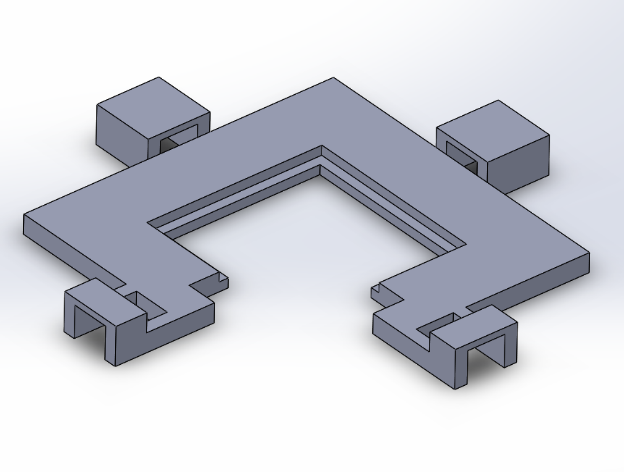
\includegraphics[width=0.6\textwidth]{2-14}
\caption{魔方托槽仿真图}\label{fig:2-14}
\end{figure}

\subsection{装配仿真图}

对于本论文提出的魔方复原系统,其装配结构对整体性能具有非常重要的影响。整个魔方还原系统需要设计多个方面的仿真结构,包括魔方与托槽装配仿真图、系统装配仿真图。

其中,下图~\ref{fig:2-15}~给出的魔方与托槽装配仿真图用于模拟仿真系统空闲时魔方放置在托槽上的状态;图~\ref{fig:2-16}~与图~\ref{fig:2-17}~的系统装配仿真图用于模拟仿真整个系统的硬件框架,在实际装配的过程中以该仿真图为参照物搭建整个系统,为整体系统搭建提供极大的便利。

\begin{figure}[H]
	\centering
	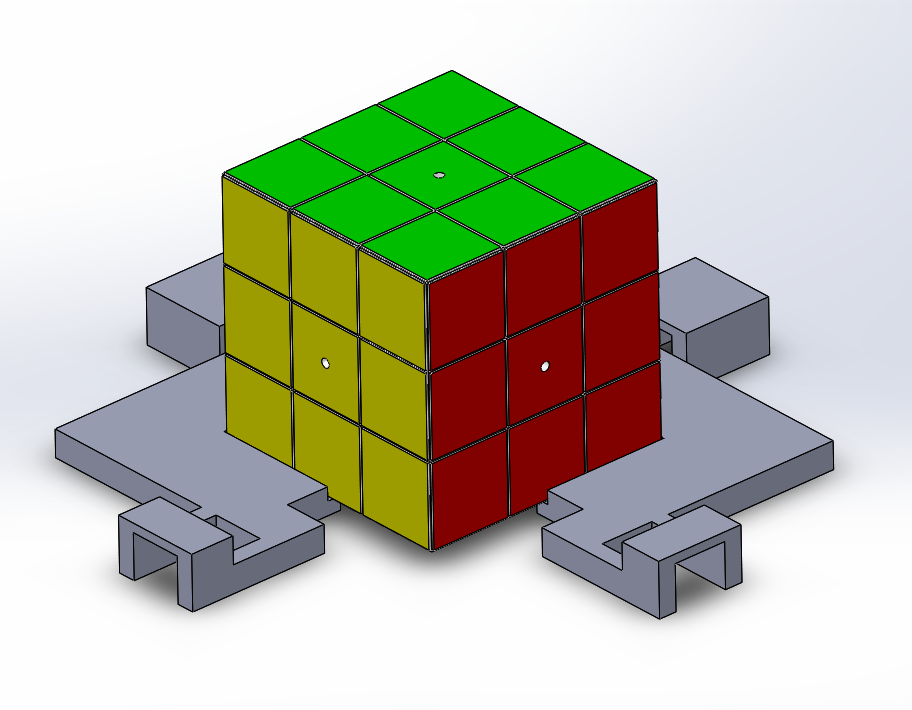
\includegraphics[width=0.6\textwidth]{2-15}
	\caption{魔方与托槽装配仿真图}\label{fig:2-15}
\end{figure}

\begin{figure}[H]
	\centering
	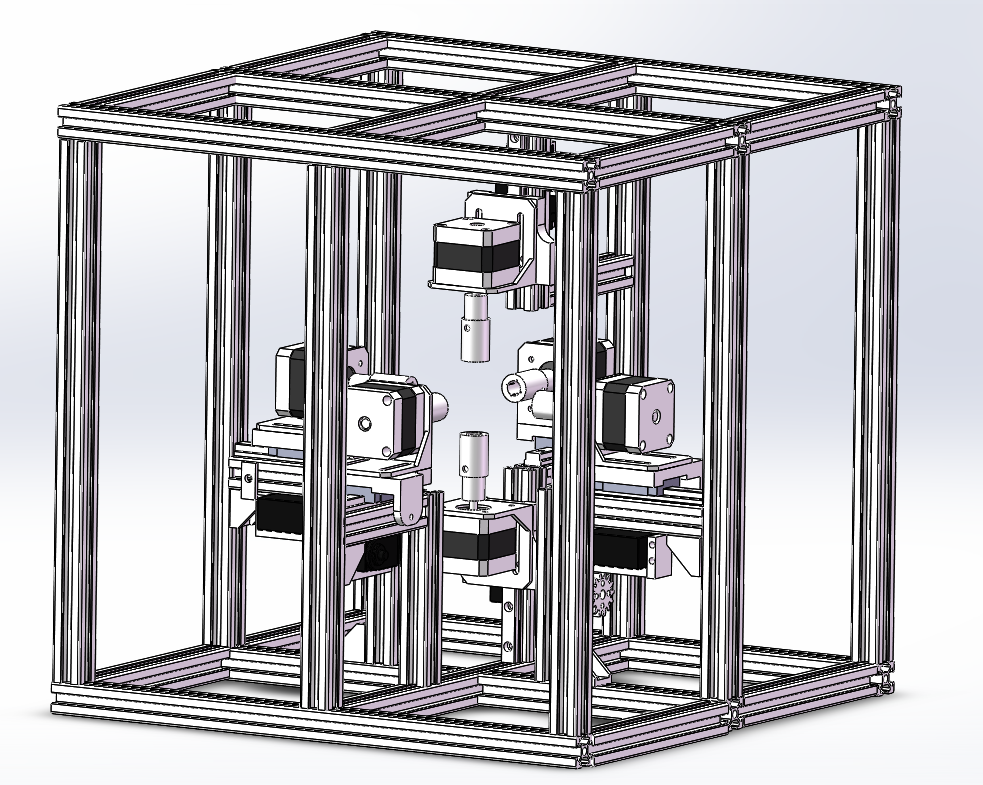
\includegraphics[width=0.6\textwidth]{2-16}
	\caption{系统装配仿真图(侧视图)}\label{fig:2-16}
\end{figure}

\begin{figure}[H]
	\centering
	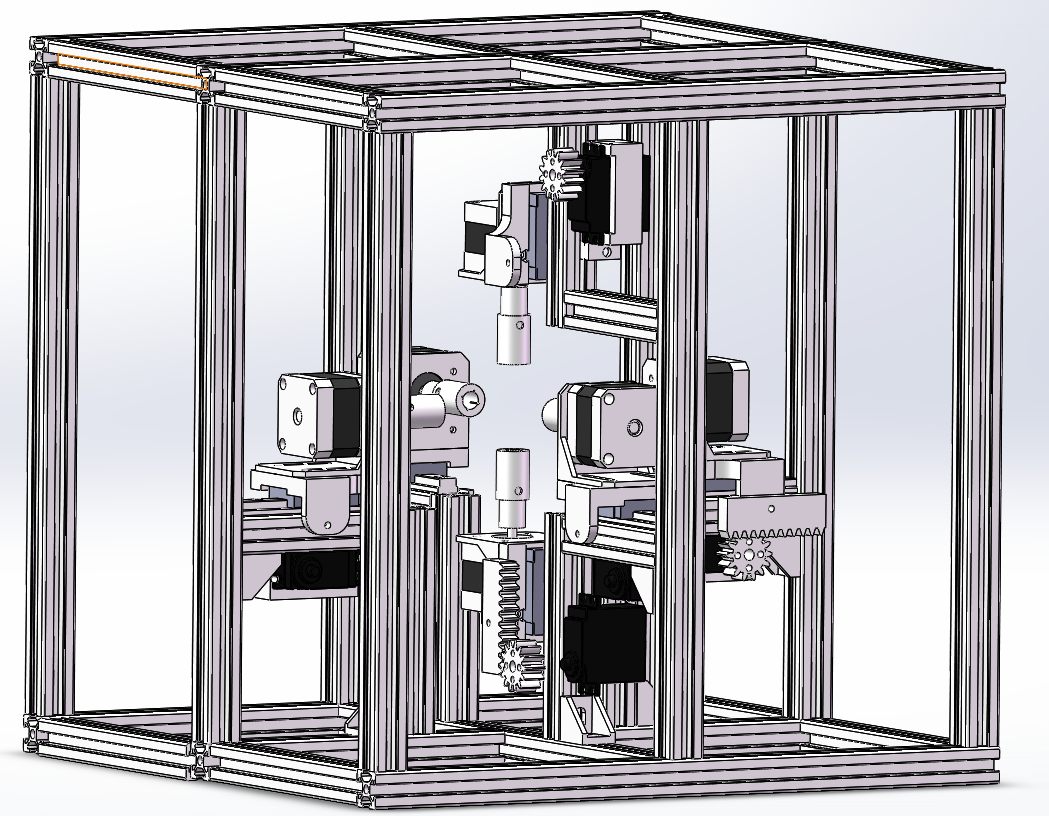
\includegraphics[width=0.6\textwidth]{2-17}
	\caption{系统装配仿真图(背视图)}\label{fig:2-17}
\end{figure}

\subsection{实际搭建效果图}

在本系统硬件部分的设计中,有一部分零件结合3D打印技术打印而成,也有一部分是使用现有相同规格的材料。图~\ref{fig:2-18}、图~\ref{fig:2-19}~为实际搭建的效果图,该框架是以上部分所示的仿真图为参照物进行系统搭建。

\begin{figure}[H]
	\centering
	\subfigure{
		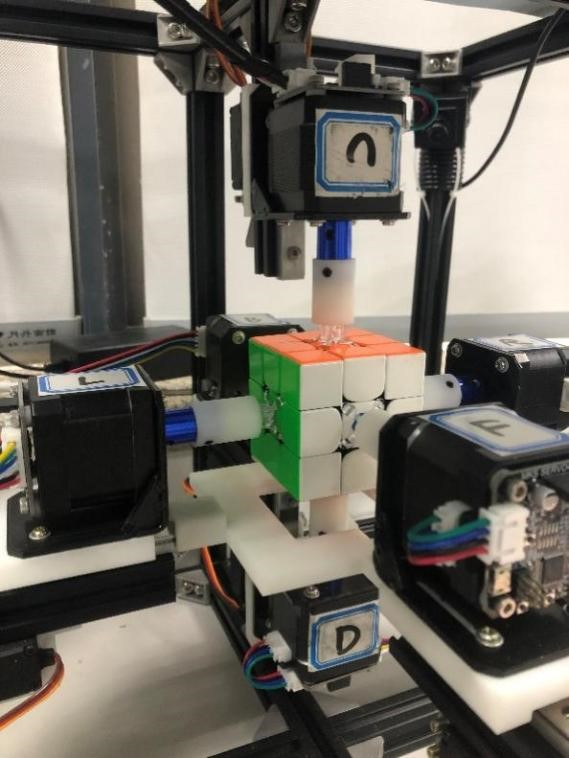
\includegraphics[width=0.4\textwidth]{2-18}}
	\subfigure{
		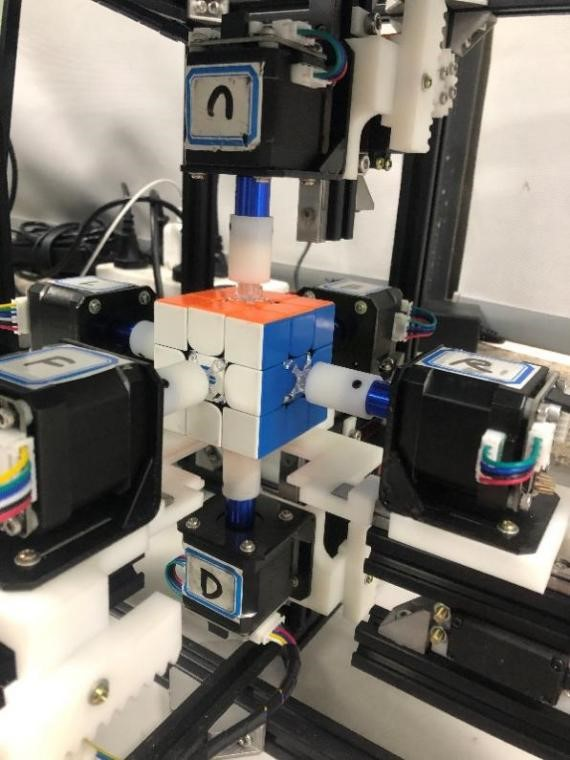
\includegraphics[width=0.4\textwidth]{2-18.1}}
	\caption{系统侧视图}\label{fig:2-18}
\end{figure}

\begin{figure}[H]
	\centering
	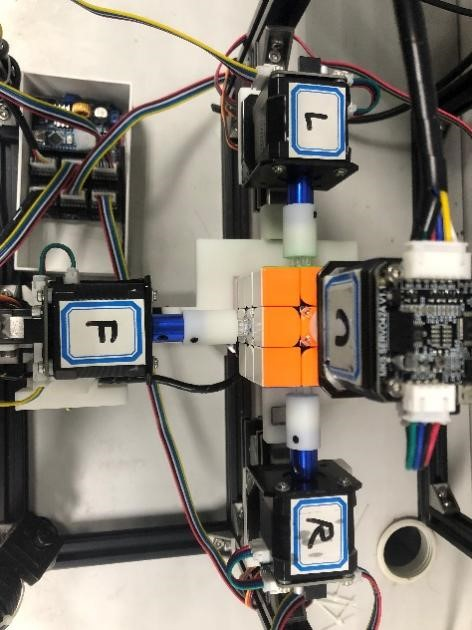
\includegraphics[angle=90,width=0.8\textwidth]{2-19}
	\caption{系统俯视图}\label{fig:2-19}
\end{figure}

\subsection{本章小结}

本章首先是介绍搭建本系统的硬件设备,接着简要阐述自主设计PCB电路板的思路,随后展示借助三维建模软件SolidWorks对魔方复原系统的框架整体搭建的建模结果图以及实际搭建后的效果图。本章列举本系统中硬件框架部分的内容,是本系统中最基础、最底层的一部分,为下一章系统软件算法的开发打下扎实的基础。